\documentclass[11pt, t]{beamer}
\usepackage{amsmath}
\usepackage{setspace}
\usepackage{float} 
\usepackage{multido}
\usepackage{multirow}
\usepackage{array}
\usepackage{enumerate}
\usepackage{booktabs}
\usepackage{indentfirst} 
\usepackage[style=mla]{biblatex}
\usepackage{setspace}
\usepackage{calligra}
\usepackage{subcaption}
\usepackage{hyperref}
\usepackage{textpos}

\makeatletter
\let\@@magyar@captionfix\relax
\makeatother

\definecolor{Turquoise3}{RGB}{0, 134, 139}
\renewcommand{\emph}[1]{{\color{Turquoise3}\textsl{#1}}}
\newcommand{\C}{\mathbb{C}} \newcommand{\F}{\mathbb{F}} \newcommand{\R}{\mathbb{R}} \newcommand{\Q}{\mathbb{Q}}
\newcommand{\N}{\mathbb{N}}
\newcommand{\myseries}[2]{$#1_1,#1_2,\dots,#1_#2$}
\newcommand{\nullspace}{~\\[15pt]}
\newcommand{\rot}{\text{\Large{\calligra{rot}}\,}}
\newcommand{\Remark}{\textbf{Remark: }}
\newcommand{\Question}{\textbf{Question: }}
\newcommand{\Extension}{\textbf{Extension: }}
\newcommand{\scp}[2]{\langle\,#1\,,\,#2\,\rangle} \newcommand{\scpp}{\langle\,\cdot\,,\,\cdot\,\rangle}


\usetheme{Madrid}
\setbeamertemplate{navigation symbols}{}

\addtobeamertemplate{frametitle}{}{
\begin{textblock*}{100mm}(0.85\textwidth,-1cm)

\includegraphics[height=1cm]{Figures/logo/logo.png}
\end{textblock*}}

\definecolor{themecolor}{RGB}{25,25,112} 

\usecolortheme[named=themecolor]{structure}

\setbeamertemplate{items}[default]

\hypersetup{
    colorlinks=true,
    linkcolor=themecolor,
    filecolor=themecolor,      
    urlcolor=themecolor,
    citecolor=themecolor,
}

\title{VV285 RC Part VII}
\subtitle{\textbf{Vector Fields}\\\large Flux, Circulation and Fundamental Theorem of Calculus}
\institute[UM-SJTU JI]{University of Michigan-Shanghai Jiao Tong University Joint Institute}
\author{Pingbang Hu}

\begin{document}

\begin{frame}
    \titlepage
    \begin{center}
        
\includegraphics[height=2cm]{Figures/logo/logo2.png}
    \end{center}
\end{frame}

\section{Flux, Circulation and Fundamental Theorem of Calculus}
\begin{frame}
    \frametitle{Outline}
    \begin{spacing}{1.2}
        \tableofcontents[currentsubsection,hideothersubsections,sectionstyle=hide]
    \end{spacing}
\end{frame}

\subsection{Overview}
\begin{frame}
    \frametitle{Overview}
    Flux, circulation, divergence, rotation, gradient,\dots The concepts we learned last week have practical significance in subject
    such as \emph{fluid dynamics} and \emph{electromagnetics}. It is important for us to be familiar with these concepts.
    \vspace{1cm}
    \begin{figure}[H]
    \centering
    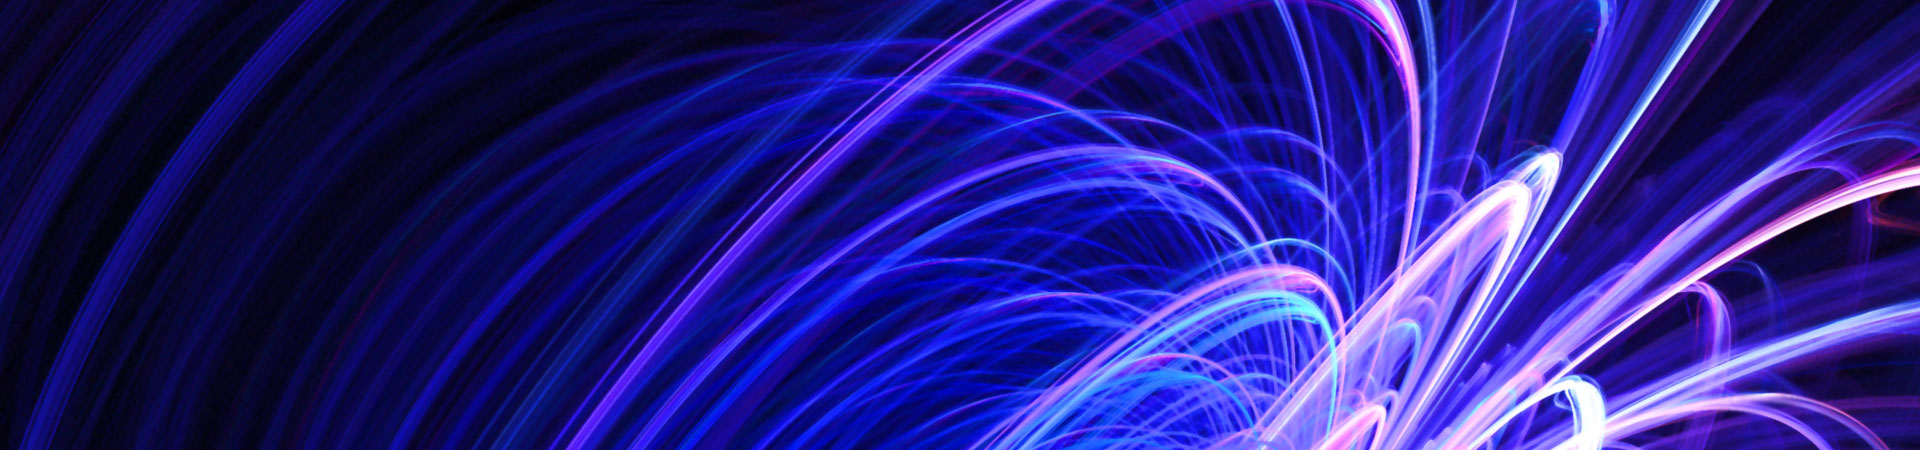
\includegraphics[width=0.9\textwidth]{Figures/2020-07-22-15-16-33.png}
    \caption{Electromagnetics}
    \end{figure}
\end{frame}

\subsection{Flux and Divergence}
\begin{frame}[allowframebreaks]
    \frametitle{Flux and Divergence}
    Let $F:\R^{n}\to\R^{n}$ be a vector field defined in a neighborhood
    of a hypersurface $\mathcal{S}$ with parametrization $\varphi:\Omega\to\R^{n},\Omega\subset\R^{n-1}$. Then we define the \emph{flux of $F$ through $\mathcal{S}$} by
    \begin{equation*}
        \begin{split}
            \int_\mathcal{S}F\,d\vec{A} &:=\int_\mathcal{S}\scp{F}{N}\,dA \qquad(=\int_\mathcal{S}\scp{F}{d\vec{A}}\,)\\
            &=\int_\Omega\scp{F\circ\varphi(x)}{N\circ\varphi(x)}\sqrt{g(x)}\,dx_1...dx_{n-1}
        \end{split}
    \end{equation*}
    And
    \[\text{div}\,F:=\frac{\partial F_1}{\partial x_1}+\cdots+\frac{\partial F_n}{\partial x_n}\]
    is called the \emph{divergence} of $F$.\\[5pt]
    \Remark The total flux density at a point $x$ is given by the divergence of the field at
    $x$.\newpage
    In triangle calculus, the divergence of a vector field $F$ can be expressed as
    \[\text{div}\,F=\scp{\nabla}{F}=\left\langle{\begin{pmatrix}
                \frac{\partial}{\partial x_1} \\
                \vdots                        \\
                \frac{\partial}{\partial x_n}
            \end{pmatrix}}{\begin{pmatrix}
                F_1    \\
                \vdots \\
                F_n
            \end{pmatrix}}\right\rangle=\frac{\partial F_1}{\partial x_1}+\cdots+\frac{\partial F_n}{\partial x_n}.\]

    In some other notations, one also uses $\nabla\cdot F$ to indicates the divergence of $F$. This type of notation is more common in a physical textbooks.
\end{frame}

\begin{frame}
    \frametitle{Exercise 1: Flux}

    Find the flux of the vector field $F: \mathbb{R}^{3} \rightarrow \mathbb{R}^{3}$,
    $
        F(x, y, z)=(x, 1, z)
    $,
    along the surface $S=\left\{(x, y, z) \in \mathbb{R}^{3}: x^{2}+z^{2} \leq 9, y=x^{2}+z^{2}\right\}$ Assume y-axis to be negative orientation. 
\end{frame}


\subsection{Circulation and Rotation/Curl}
\begin{frame}[allowframebreaks]
    \frametitle{Circulation and Rotation/Curl}

    Let $\Omega\subset\R^n$ be an open set, $F:\Omega\to\R^n$ a continuously dif{}ferentiable vector field and $\mathcal{C}^*$ an oriented closed curve in $\R^n$. Then
    \begin{equation*}\label{3.2.1}
        \int_{\mathcal{C}^*}\scp{F}{T}\,ds
    \end{equation*}
    is called the (total) \emph{circulation} of $F$ along $\mathcal{C}$. Then the anti-symmetric, bilinear form
    \begin{equation*}\label{3.2.3}
        \rot F|_x:\R^n\times\R^n\to\R,\qquad
        \rot F|_x(u,v):=\scp{DF|_xu}{v}-\scp{DF|_xv}{u}
    \end{equation*}
    is called the \emph{rotation} (in mainland Europe) or \emph{curl} (in anglo-saxon countries) of the vector field $F$ at $x\in\R^n$.
    \newpage
    Let $\Omega\subset\R^2$ be open and $F:\Omega\to\R^2$ a continuously dif{}ferentiable vector field. Then here exists a uniquely defined continuous \textbf{potential} function $\text{rot}\,F:\Omega\to\R$ such that
    \begin{equation*}\label{3.2.5}
        \rot\,F|_x(u,v)=\text{rot}\,F(x)\cdot
        \det(u,v).
    \end{equation*}
    Moreover, $$\text{rot}\,F(x)=\frac{\partial F_2}{\partial x_1}-\frac{\partial F_1}{\partial x_2}.$$
    \Remark $\text{rot}\,F$ represents the circulation density in $\R^2$.
    \newpage
    Let $\Omega\subset\R^3$ be open and $F:\Omega\to\R^3$ a continuously dif{}ferentiable vector field. Then here exists a uniquely defined continuous \textbf{vector} field $\text{rot}\,F:\Omega\to\R^3$ such that
    \begin{equation*}\label{3.2.7}
        \rot\,F|_x(u,v)=\scp{\text{rot}\,F(x)}{u\times v}=\det(\text{rot}\,F(x),u,v).
    \end{equation*}
    Moreover, \[\text{rot}\,F(x)=\begin{pmatrix}
            \frac{\partial F_3}{\partial x_2}-\frac{\partial F_2}{\partial x_3} \\[4pt]
            \frac{\partial F_1}{\partial x_3}-\frac{\partial F_3}{\partial x_1} \\[4pt]
            \frac{\partial F_2}{\partial x_1}-\frac{\partial F_1}{\partial x_2}
        \end{pmatrix}.\]
    \Remark $\text{rot}\,F$ represents the circulation density in $\R^3$.\nullspace
    A simply connected innovational vector field is a potential field.
    \newpage
    In triangle calculus, the rotation of a vector field $F$ can be formally written as
    \[\text{rot}\,F=\nabla\times F(x)
        =\det\begin{pmatrix}
            e_1                           & e_2                           & e_3                           \\[3pt]
            \frac{\partial}{\partial x_1} & \frac{\partial}{\partial x_2} & \frac{\partial}{\partial x_3} \\[3pt]
            F_1                           & F_2                           & F_3
        \end{pmatrix},\]
    where $e_1,e_2,e_3$ are the standard basis vectors in $\R^3$.
    \nullspace
    \Remark The triangle notation is a good mnemonics to help us memorize these formulas. (Why?)
\end{frame}

\begin{frame}
    \frametitle{Exercise 2 \& 3: Circulation \& Potential}
    Let $G(x, y)=\left(2 x y e^{x^{2}}+\frac{y}{x}, e^{x^{2}}+\ln x+6 y\right)$ be a vector field in $\R^2$, $G:\{(x,y):x>0,y>0\}\to\R^2$.
    \begin{itemize}
        \item Is $G$ a potential field?
        \item If so, find the form of its potential function. Otherwise, prove it's not conservative.
    \end{itemize}
    \vspace{1cm}
    Let $F(x,y,z)=(e^z,1,xe^z)$ be a vector field in $\R^3$.
    \begin{itemize}
        \item Is $F$ a potential field?
        \item If so, find the form of its potential function. Otherwise, prove it's not conservative.
    \end{itemize}

\end{frame}




\subsection{Green's Theorem}
\begin{frame}
    \frametitle{Green's Theorem}
    Let $R\subset\R^2$ be a bounded, simple region and $\Omega\supset R$ an open set containing $R$. Let $F:\Omega\to\R^2$ be a continuously dif{}ferentiable vector field. Then
    \setcounter{equation}{0}
    \begin{equation*}\label{3.4.1}
        \int_{\partial R^*}F\,d\vec{s}=\int_R\left(\frac{\partial F_2}{\partial x_1}-\frac{\partial F_1}{\partial x_2}\right)\,dx
    \end{equation*}
    where $\partial R^*$ denotes the boundary curve of $R$ with positive
    (counter-clockwise) orientation.\\[9pt]

    \Remark Green's theorem is basically a particular case of Stokes's theorem. A clever use of it is to calculate the area of a simple region. For $F(x_1,x_2)=(-x_2,x_1)$ we obtain
    \[|R|=\int_R1\,dx=\frac{1}{2}\int_{\partial R}\binom{-x_2}{x_1}d\vec{s}.\]
    For a bounded simple region, the value along the boundary contains the information of the area.
\end{frame}

\begin{frame}
    \frametitle{Exercise 4: Green's Theorem}
    Find the area of region $R$ that is bounded by the curve $\mathcal{C}$, whose parametrization is % The answer is 4/3
    $$\gamma(t)=\begin{pmatrix}
            \sin 2t \\\sin t
        \end{pmatrix},\quad t\in[0,\pi].$$
    \begin{figure}[H]
        \centering
        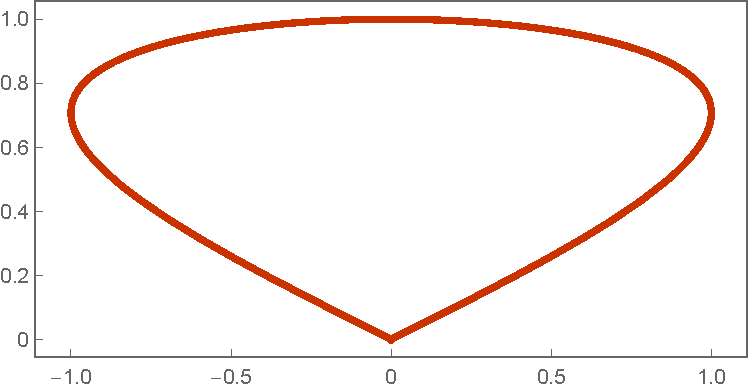
\includegraphics[width=0.6\textwidth]{Figures/p1.pdf}
    \end{figure}
\end{frame}

\subsection{Gau\ss's Theorem}
\begin{frame}
    \frametitle{Gau\ss's Theorem}
    Let $R\subset\R^n$ be an admissible region and $F:\overline{R}\to\R^n$ a continuously dif{}ferentiable vector field. Then
    \[\int_R\text{div}\,F\,dx=\int_{\partial R^*}F\,d\vec{A}.\]
\end{frame}

\begin{frame}
    \frametitle{Exercise 5: Gau\ss's Theorem}
    Calculate the integral
    \[
        \int_{S^{2}}(x y+y z+z x) d \sigma
    \]
    where $S^{2}=\left\{(x, y, z) \in \mathbb{R}^{3}: x^{2}+y^{2}+z^{2}=1\right\}$ is the unit sphere.
\end{frame}

\begin{frame}
    \frametitle{Exercise 6: Gau\ss's Theorem}
    Let $F: \mathbb{R}^{3} \rightarrow \mathbb{R}^{3}, F(x, y, z)=(x, y, z)$ and
    \[
        U=\left\{(x, y, z) \in \mathbb{R}^{3}: x^{2}+y^{2} \leq 1, x+z \leq 2, z \geq 0, x \geq 0\right\}
    \]
    Denote by $S=\partial U$ the surface of $U$ and by $N$ the outward-pointing unit normal vector on $S .$ Let $S^{+}$ denote the surface $S$ with positive orientation.
    \begin{itemize}
        \item Sketch $U$.
        \item Calculate the flux $\int_{S^{+}}\langle F, N\rangle d \sigma$
    \end{itemize}
\end{frame}




\subsection{Stokes's Theorem}
\begin{frame}
    \frametitle{Stokes's Theorem}
    Let $\Omega\subset\R^3$ be an open set, $\mathcal{S}\subset\Omega$ a parametrized, admissible surface in $\R^3$ with boundary $\partial\mathcal{S}$ and let $F:\Omega\to\R^3$ be a continuously dif{}ferentiable vector field. Then
    \[\int_{\partial\mathcal{S}^*}F\,d\vec{s}=
        \int_{\mathcal{S}^*}\text{rot}\,F\,d\vec{A}\]
    where the orientations of the boundary curve $\partial\mathcal{S}^*$ and the surface $\mathcal{S}^*$ are chosen according to \emph{right hand law}.
\end{frame}

\begin{frame}
    \frametitle{Exercise 7: Stokes's Theorem}
    Let $\mathcal{C}$ be the curve illustrated below.
    \begin{figure}[H]
        \centering
        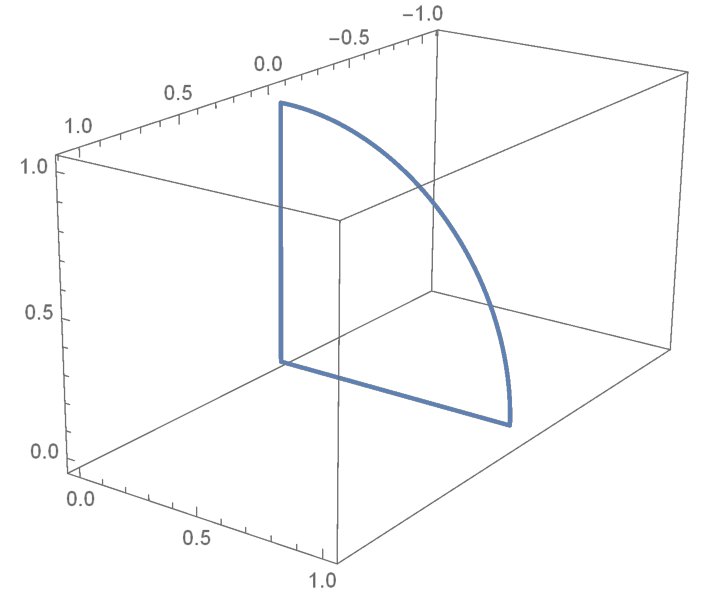
\includegraphics[width=0.4\textwidth]{Figures/p2.pdf}
    \end{figure}
    For $F(x,y,z)=(y,z,x)$, compute the circulation along $\mathcal{C}$ using Stokes's theorem.
\end{frame}

\begin{frame}
    \frametitle{Exercise 8: Stokes's Theorem}
    Let $${F}(x, y, z)=\left(\sin x-\dfrac{y^{3}}{3}, \cos y+\dfrac{x^{3}}{3}, x y z\right).$$ Calculate the circulation of $F$ along $\mathcal{C}$, where $\mathcal{C}$ is the oriented unit circle in the plane $z=1$. (The orientation is counter-clockwise if viewing from positive z-axis).
    \begin{figure}[H]
        \centering
        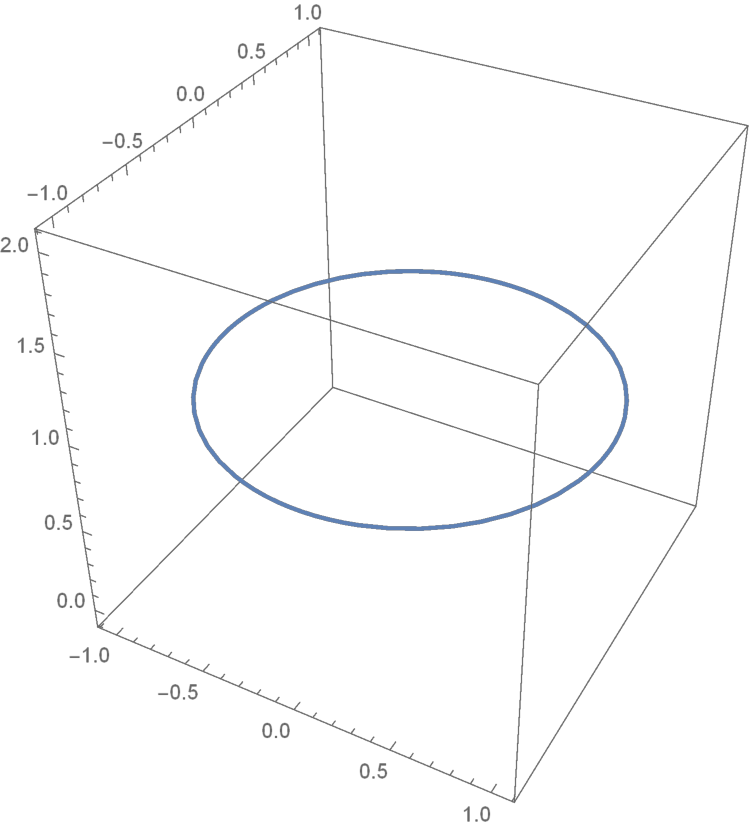
\includegraphics[width=0.3\textwidth]{Figures/p3.pdf}
    \end{figure}
\end{frame}

\begin{frame}
    \frametitle{Application 1: Electromagnetics}
    \begin{tabular}{l l}

        \textit{Integral Equations}                                                                                                                                                                                & \textit{Differential Equations}                                                             \\
        $\displaystyle\oint_{\partial \Omega} {E} \cdot \mathrm{d} {S}=\frac{1}{\varepsilon_{0}} \int_{\Omega} \rho \mathrm{d} V$                                                                                  & $\displaystyle\nabla \cdot {E}=\frac{\rho}{\varepsilon_{0}}$                                \\
        $\displaystyle\oint_{\partial \Omega} {B} \cdot \mathrm{d} {S}=0$                                                                                                                                          & $\displaystyle\nabla \cdot {B}=0$                                                           \\
        $\displaystyle\oint_{\partial \Sigma} {E} \cdot \mathrm{d} \ell=-\frac{\mathrm{d}}{\mathrm{d} t} \int_{\Sigma} {B} \cdot \mathrm{d} {S}$                                                                   & $\displaystyle\nabla \times {E}=-\frac{\partial {B}}{\partial t}$                           \\
        $\displaystyle\oint_{\partial \Sigma}{B} \cdot {d} \ell=\mu_{0}\left(\int_{\Sigma} {J} \cdot \mathrm{d} {S}+\varepsilon_{0} \frac{\mathrm{d}}{\mathrm{d} t} \int_{\Sigma} {E} \cdot \mathrm{d} {S}\right)$ & $\nabla \times {B}=\mu_{0}\left({J}+\varepsilon_{0} \frac{\partial {E}}{\partial t}\right)$
        \\
    \end{tabular}
    \vspace{10pt}

    The famous equations above are called the \emph{Maxwell equations}. They together describe fundamental behaviors of electromagnetic fields. Can you find the relations between the integral equations and differential equations?
\end{frame}

\subsection{*Vector Calculus Identity}
\begin{frame}
    \frametitle{Exercise 9: *Vector Calculus Identity}
    As we have discussed last week, physicists really love using triangle notations because this good notation makes life easier. See those common equalities in vector calculus, and think about what they indicate/why they hold/why the triangle notations are user-friendly:
    \begin{itemize}
        \item $\nabla\times(\nabla f)=0$
        \item $\nabla\cdot(\nabla\times F)=0$
        \item $\nabla \times\left(\dfrac{F}{\phi}\right)=\dfrac{\phi \nabla \times F-\nabla \phi \times F}{\phi^{2}}$
    \end{itemize}
    \vspace{10pt}
    \Remark In electromagnetics, we define \emph{magnetic vector potential} $A$ to be a vector field such that 
    $$B=\nabla\times A$$ and \emph{electric potential} $\phi$ to be scalar field such that $$E=-\nabla \phi -\dfrac{\partial A}{\partial t}.$$
    How does such a definition correspond with Maxwell equations?
\end{frame}

\subsection{Green's Identity}
\begin{frame}
    \frametitle{Green's Identity}
    Let $R\subset\R^n$ be an admissible region and $u,v:\overline{R}\to\R$ be twice continuously dif{}ferentiable potential functions. Then
    \begin{equation}\label{3.6.4}
        \int_R\scp{\nabla u}{\nabla v}\,dx=-\int_R u\cdot\Delta v\,dx+\int_{\partial R^*}u\frac{\partial v}{\partial n}\,dA
    \end{equation}
    and
    \begin{equation}\label{3.6.5}
        \int_R(u\cdot\Delta v-v\cdot\Delta u)\,dx=\int_{\partial R^*}\left(u\frac{\partial v}{\partial n}-v\frac{\partial u}{\partial n}\right)\,dA.
    \end{equation}
    \\[16pt]
    \eqref{3.6.4} is commonly called \emph{Green's first identity} and \eqref{3.6.5} \emph{Green's second identity}.\\[9pt]
\end{frame}

\begin{frame}
    \frametitle{Application 2: Fluid Dynamics}
    The properties of the Laplace operator $\Delta$ acting on smooth functions defined on some set $\Omega \subset \mathbb{R}^{n}$ are important in the theory of differential equations. Green's identities are your friend here:
    \nullspace
    Let $\Omega \subset \mathbb{R}^{2}$ be an open, bounded, connected set and $u: \Omega \rightarrow \mathbb{R}$ a twice differentiable function such that
    \[
        \frac{\partial^{2} u}{\partial x_{1}^{2}}+\frac{\partial^{2} u}{\partial x_{2}^{2}}=0
    \qquad and \qquad
        \left.\frac{\partial u}{\partial n}\right|_{\partial \Omega}=0
    \]
    \begin{enumerate}
        \item Prove that $u$ is constant, i.e., there exists some $c \in \mathbb{R}$ such that $u(x)=c$ for all $x \in \Omega$.
        \item Interpret the statement of this exercise physically in terms of fluid flow (potential flow) in a container.
    \end{enumerate}
\end{frame}

\begin{frame}
    \frametitle{Extra}
    \vfill
    \begin{center}
        \LARGE
        Enjoy the following!
    \end{center}
    \vfill
\end{frame}

\end{document}